\section{Studio dei punti fissi della mappa logistica}
Una volta visto cosa rappresentano i punti fissi di una funzione e alcune loro caratteristiche, si può finalmente tornare al problema della descrizione della dinamica di una popolazione, e cercare i punti fissi della mappa logistica scelta per descriverla. Allo scopo di analizzarla con più facilità dal punto di vista analitico, può essere comodo d'ora in poi scrivere l'equazione logistica in forma continua, vale a dire nella forma
\begin{equation}
    f(x) = rx(1-x) = rx - rx^2
    \label{eq:logistica_continua}
\end{equation}
Si tratta dunque di una famiglia di infinite funzioni, che dipendono dal parametro $r$. Nella figura \ref{fig:logistiche} sono state rappresentate alcune di queste funzioni al variare di $r$.

Da un punto di vista rigoroso l'operazione di rendere continua la mappa logitica discreta deve essere fatta con cautela, dal momento che i valori di $x$, nel caso di una popolazione composta da un numero intero di invidui, possono essere razionali ma non irrazionali. Dal punto di vista della trattazione, tuttavia, lavorare con funzioni definite sui reali permette di usare gli strumenti dell'algebra e dell'analisi che sono di grande utilità. Si studierà quindi il comportamento dell'equazione logistica da un punto di vista più astratto, tenendo presente queste osservazioni nel caso in cui si intendano applicare i risultati ad una vera popolazione.\\
\begin{figure}[h!]
    \begin{center}
    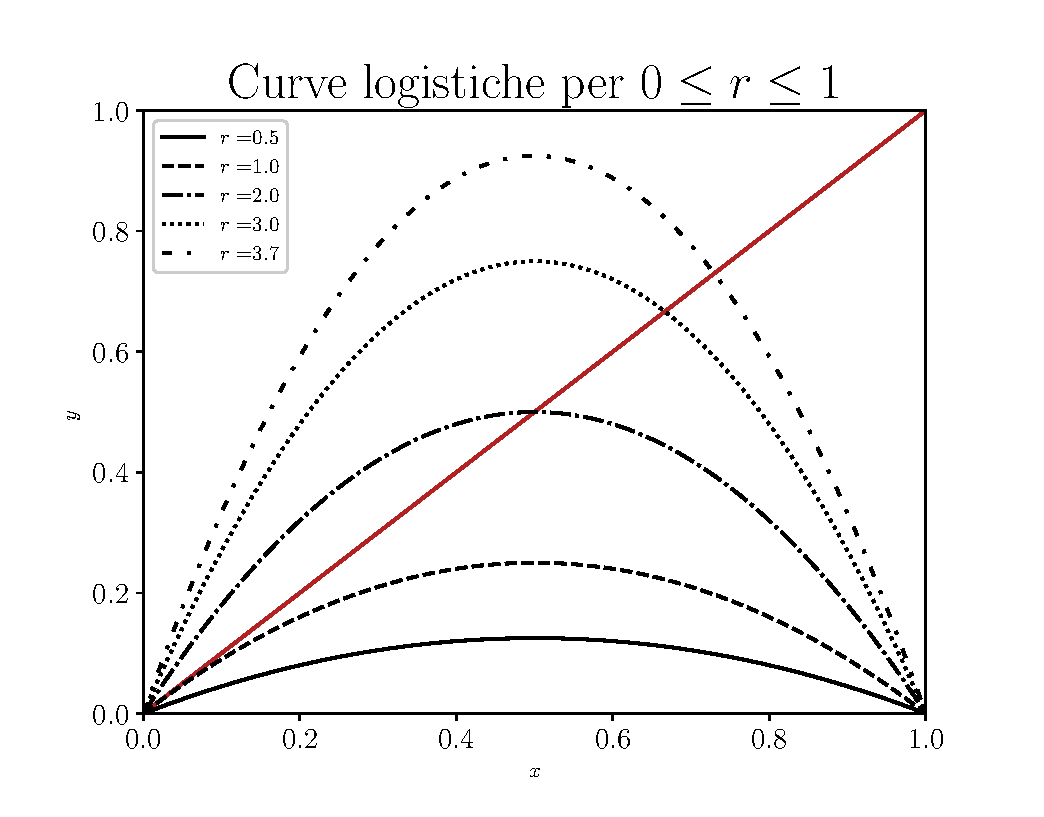
\includegraphics[scale=0.65]{Immagini/curve_logistiche.eps}
    \captionsetup{width=.8\linewidth}
    \caption{Curva logistica per diversi valori del parametro $r$. È stata tracciata anche la bisettrice in rosso, che sarà utile per individuare i punti fissi.}
    \label{fig:logistiche}
    \end{center}
\end{figure}

Si vuole dunque studiare quali sono i punti fissi della funzione \ref{eq:logistica_continua} nell'intervallo di interesse $[0,1]$ al variare del parametro $r$. Innanzitutto bisogna osservare che, se il valore di $f$ deve rimanere all'interno dell'intervallo $[0,1]$, $r$ non può ammettere valori arbitrari. Dalla figura \ref{fig:logistiche} si osserva che il valore massimo assunto dalla funzione logistica dipende dal valore di $r$ e si trova in corrispondenza del vertice; calcolando che l'ordinata del vertice corrisponde a $r/4$, e imponendo che questo sia compreso tra 0 e 1 (inclusi, dato che gli estremi sono valori ammessi), si ottiene la condizione 
\[
    \boxed{0 \leq r \leq 4}
\]
Una volta appurato ciò, si possono calcolare facilmente i punti fissi della funzione \ref{eq:logistica_continua} risolvendo in modo algebrico l'equazione $$ x = rx - rx^2$$ le cui soluzioni generali sono 
\[
    \boxed{x_{eq,1} = 0} \quad \boxed{x_{eq,2} = 1 - \dfrac{1}{r}}
\]
L'interesse è ora quello di studiare la natura di questi punti fissi al variare di $r$. A tal fine, può essere utile riportare qui anche la funzione derivata di f, che verrà utilizzata più volte in seguito:
\begin{equation}
    \dfrac{\dif f(x)}{\dif x} = r (1-2x)
    \label{eq:derivata}
\end{equation}
\subsection{Punti fissi per $0\leq r \leq 1$}
Per valori di $r$ compresi tra 0 e 1, $x_{eq,2}$ risulta minore di 0, dunque non è un valore ammesso e si considera soltanto il punto fisso $x_{eq,1} = 0$. Si osservi che, graficamente, questo si traduce nell'avere un solo punto di intersezione tra la curva logistica e la bisettrice nell'intervallo di interesse, come si verifica nella figura \ref{fig:logistiche_r_minore_1}. 
\begin{figure}[h!]
    \begin{center}
        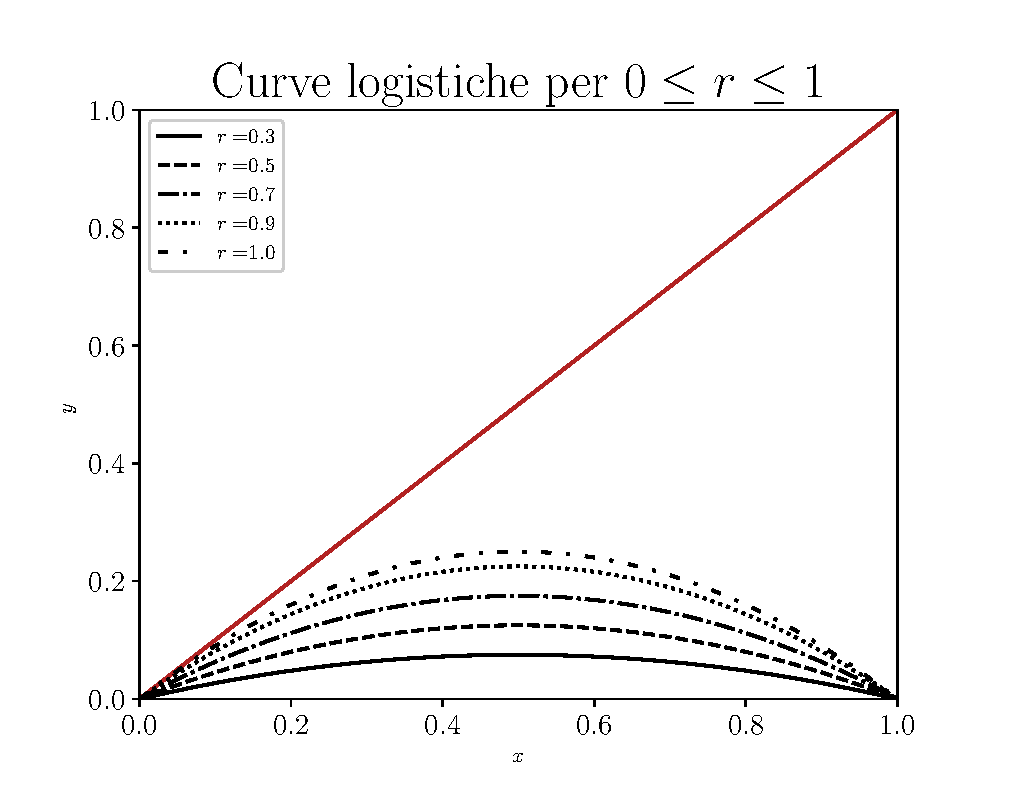
\includegraphics[scale=0.7]{Immagini/curve_logistiche_r_minore_1.eps} 
    \captionsetup{width=.8\linewidth}
    \caption{Diverse curve logistiche per $0\leq r \leq 1$. Si osserva in particolare che c'è una sola intersezione tra le curve e la bisettrice, $x = 0$, che è l'unico punto fisso per i valori considerati di $r$.}
    \label{fig:logistiche_r_minore_1}
    \end{center}
\end{figure}

La derivata di $f$ calcolata in $x = 0$ risulta essere pari a $r$. Per $r < 1$ si ha quindi la certezza che $x_{eq,1} = 0$ sia un punto fisso attrattore, come è ragionevole supporre se si pensa che per $r<1$ la popolazione non può che diminuire a ogni iterazione, fino a estinguersi. Non è possibile usare il metodo della derivata per $r = 1$ invece, ma ci si rende facilmente conto che iterando la funzione $f(x) = x - x^2$ partendo da valori di $x$ compresi tra 0 e 1, si ottiene una successione decrescente di valori convergente a 0; quindi $x_{eq,1} = 0$ è punto fisso attrattivo anche per $r = 1$. Nella figura \ref{fig:r1} si possono osservare diverse successioni per $r=1$ partendo da diversi valori di $x$, tutte convergenti a 0.

\begin{figure}[h!]
    \begin{center}  
    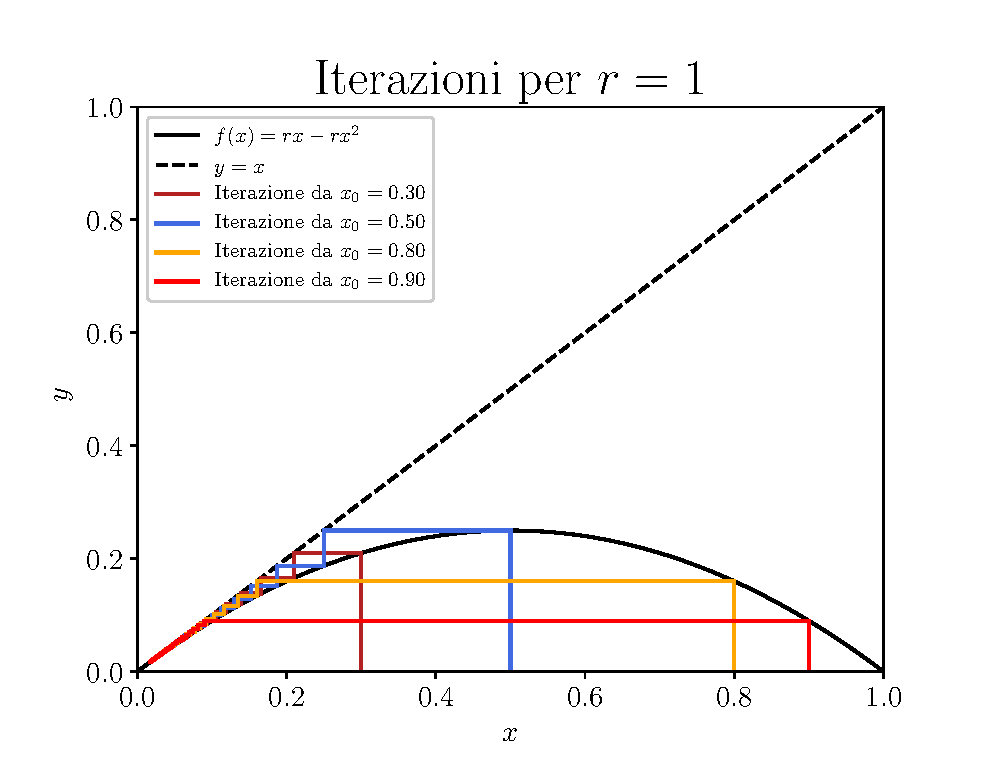
\includegraphics[scale=0.7]{Immagini/iterazioni_r1.eps} 
    \captionsetup{width=.8\linewidth}
    \caption{Iterazioni della funzione logistica per $r=1$, a partire da diversi valori iniziali, convergono sempre a 0.}
    \label{fig:r1}
    \end{center}   
\end{figure}

\subsection{Punti fissi per $1 < r \leq 3$}
Per $1 < r < 3$, il punto fisso $x_{eq,1} = 0$ diventa un punto fisso repulsivo: infatti la derivata di $f$ in $x_{eq,1}$, come si è visto, vale $r$, che ora è maggiore di 1.

Adesso, inoltre, il valore dell'altro punto fisso $x_{eq,2} = 1 - 1/r$ è un valore ammissibile, e si può studiarne la natura. La derivata di $f$ calcolata in $x_{eq,2}$ vale $$ \left.\dfrac{\dif f(x)}{\dif x}\right\vert_{x_{eq,2}} = 2 -r$$ 
che risulta sempre minore di 1 in valore assoluto per $1 < r < 3$, quindi $x_{eq,2}$ è ora un punto fisso attrattore. 
Il caso $r=3$ non è risolvibile tramite lo studio della derivata, perché presso $x_{eq,2}$ essa vale $-1$. Attraverso il metodo delle iterazioni si trova che le successioni convergono sempre verso $x_{eq,2}$, ma con estrema lentezza. Nella figura \ref{fig:r3} è stato raffigurato il risultato del metodo delle iterazioni applicato ad $f$ con $r=3$ dopo 1000 iterazioni, dove si osserva che nonostante l'elevato numero di iterazioni, ancora si distinguono lo stato del sistema e punto di convergenza.
\begin{figure}[h!]
    \begin{center}  
    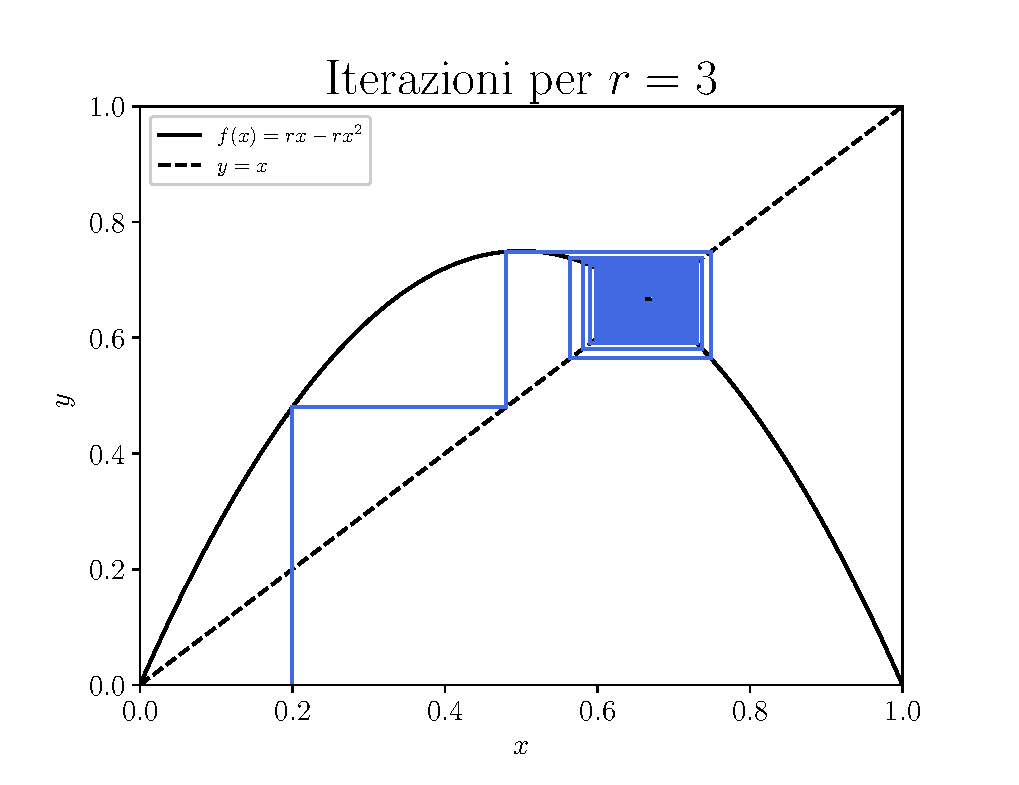
\includegraphics[scale=0.65]{Immagini/iterazioni_r3.eps} 
    \captionsetup{width=.8\linewidth}
    \caption{Iterazioni della funzione logistica per $r=3$. Per non sovraccaricare inultimente il grafico, si è scelto di raffigurare la convergenza a partire da un solo valore iniziale, ma la situazione si ripresenterebbe uguale anche partendo da un qualsiasi altro valore. Si nota come la convergenza attorno a $x_{eq,2}$ sia molto lenta, in particolare come il punto di equilibrio e lo stato del sistema dopo 1000 iterazioni siano ancora distinguibili sulla scala visualizzata, al contrario di figure precedenti.}
    \label{fig:r3}
    \end{center}   
\end{figure}

Ricapitolando il risultato di questi due ultimi paragrafi, si è trovato che quando $r$ è inferiore a 1 la popolazione è irrimediabilmente destinata a estinguersi, a prescindere dal valore iniziale. Quando $r$ invece diventa maggiore di 1, ma inferiore o uguale a 3, la popolazione cresce a partire da valori iniziali piccoli, o decresce a partire da valori iniziali grandi, fino a raggiungere asintoticamente il valore $1-1/r$, per mantenersi stabile in questo stato. Per $r=3$, tuttavia, la convergenza risulta estremamente lenta. Come si vedrà adesso, la situazione cambia radicalmente per $r > 3$.

\subsection{Punti fissi per $3 < r \leq 4$: verso il caos}
\begin{figure}[h!]
    \begin{center}
        \subfigure[]{\label{fig:osc_a} 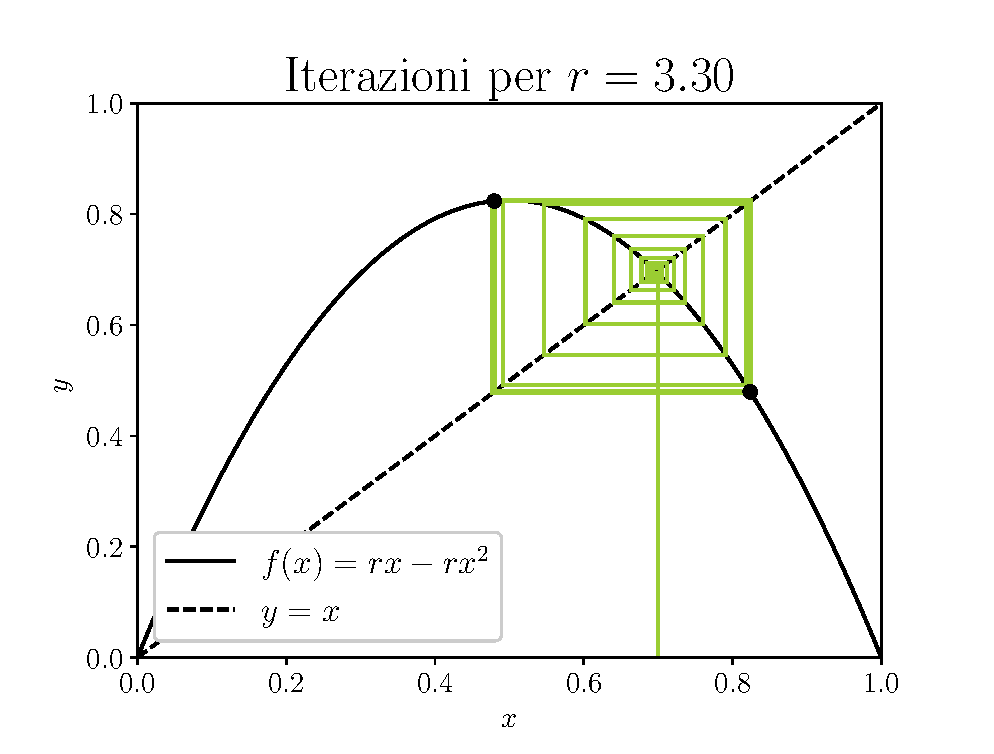
\includegraphics[scale=0.45]{Immagini/oscillazioni_1.eps}}
        \subfigure[]{\label{fig:osc_b} 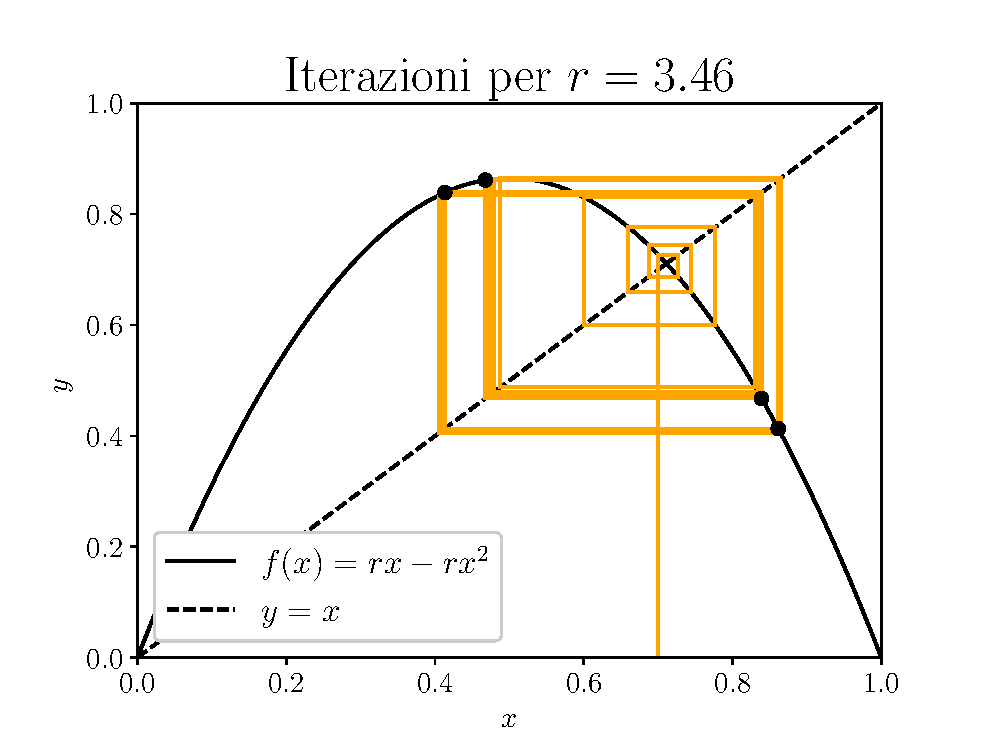
\includegraphics[scale=0.45]{Immagini/oscillazioni_2.eps}}
        \subfigure[]{\label{fig:osc_c} 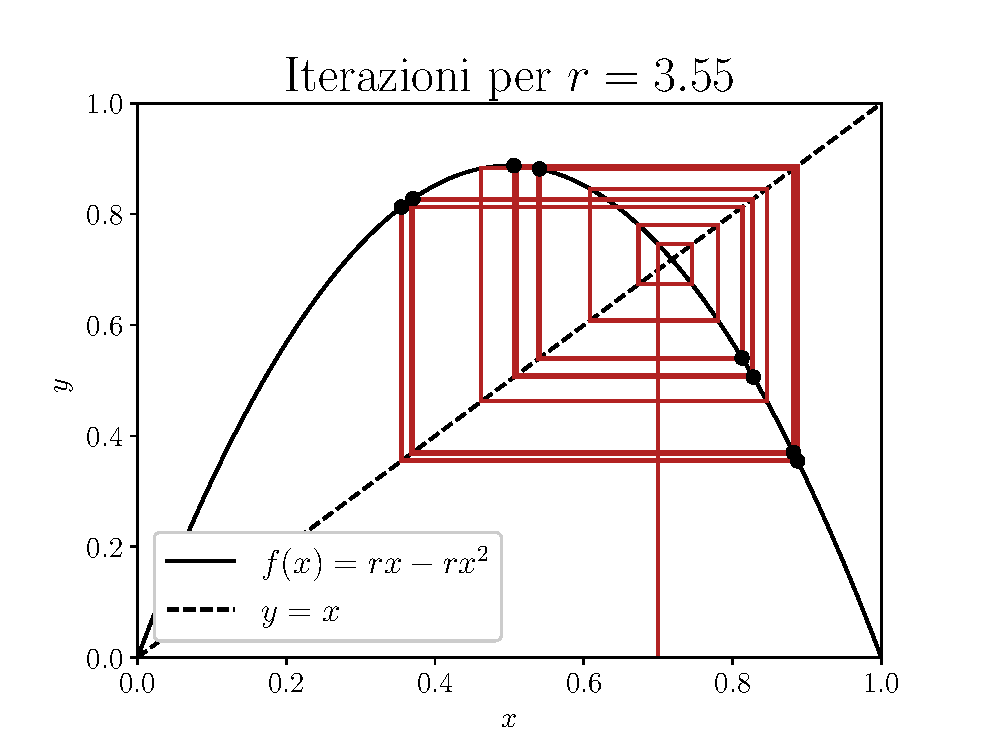
\includegraphics[scale=0.45]{Immagini/oscillazioni_3.eps}}
        \captionsetup{width=.8\linewidth}   
    \caption{Per $r > 3$ il sistema non evolve più convergendo a un valore, ma oscilla tornando periodicamente sugli stessi punti, il cui numero dipende dal valore di $r$. Nelle tre figure sono stati rappresentati, nell'ordine, i casi in cui il sistema oscilla tra 2, 4 e 16 valori. Si sono fatte partire le iterazioni dallo stesso valore, $0.7$.}
    \label{fig:oscillazioni}
    \end{center}
\end{figure}

Per $3 < r \leq 4$, sfruttando i calcoli effettuati selle sezioni precedenti, si ottiene che sia $x_{eq,1}$ che $x_{eq,2}$ sono punti fissi repulsori. Cosa succede quindi alla popolazione, se sembra che non ci siano dei valori a cui essa può tendere asintoticamente? In realtà, ci si rende conto che esistono dei punti fissi per la cosiddetta \textit{iterata seconda} di $f$, vale a dire 
\begin{equation*}
f^2(x) := f(f(x)) = r^2 x (1-x) (rx^2 -rx +1)
\end{equation*}
La funzione $f^2(x)$ è una quartica e ha quattro punti fissi, vale a dire soluzioni dell'equazione 
\begin{equation*}
    f^2(x) = x \quad \Rightarrow \quad x (r^2 (1-x) (rx^2 -rx +1) - 1) = 0
\end{equation*}
Due soluzioni sono ovviamente $x_{eq,1}$ e $x_{eq,2}$ viste fin'ora, le altre due invece sono 
\[
    \boxed{x_{eq,3,4} = \dfrac{r +1 \pm \sqrt{r^2 -2r -3}}{2r}}
\]
Calcolando la derivata di $f^2(x)$, si trova che nei due punti $x_{eq,3,4}$ la derivata assume lo stesso valore, il quale può essere, in modulo, sia maggiore che minore di 1 per $ 3 < r \leq 4$. 

Consideriamo prima il caso in cui la derivata risulti in modulo minore di 1, e quindi ci siano punti fissi attrattori per $f^2$. Si calcola che questa situazione si verifica per tutte le $r$ tali che $$ 3 < r \leq 1 +\sqrt{6}$$
Chiamiamo $r_1 := 1 +\sqrt{6} \simeq 3.449$. Dal punto di vista dell'evoluzione del sistema, queste due soluzioni rappresentano degli stati tra i quali il sistema, dopo infinite iterazioni, continua a oscillare, tornando su ciascuno di essi ogni due iterazioni di $f$: se a un certo istante il sistema si trova in corrispondenza di $x_{eq,3}$, all'iterazione successiva si troverà in $x_{eq,4}$, alla successiva di nuovo in $x_{eq,3}$, e così via. Il fatto che essi siano attrattori indica che il sistema, partendo da un certo valore iniziale, evolve tendendo asintoticamente a oscillare tra essi. Tale comportamento è visibile graficamente nella figura \ref{fig:osc_a}.


Quando invece $r_1 < r \leq 4$ la derivata di $f^2$ in $x_{eq,3,4}$ diventa maggiore di 1, e questi punti diventano quindi fissi repulsori; il sistema non evolve più tendendo a oscillare tra essi asintoticamente. Si verifica però che esistono 4 nuovi punti fissi per l'\textit{iterata terza} di $f$, $f^3$, che risultano attrattori però solo per valori di $r$ compresi tra $r_1$ e un nuovo valore $r_2 \simeq 3.544$. Per tali valori di $r$, all'infinito il sistema oscilla periodicamente tra i 4 punti fissi di $f^3$, tornando su ciascuno di essi ogni 4 iterazioni di $f$: si dice che il \textit{periodo di oscillazione} è pari a 4.

Quando $r$ supera il valore $r_2$, i quattro punti trovati diventano instabili, ma si trovano 8 nuovi punti fissi per l'iterata quarta di $f$, $f^4$, tra i quali il sistema oscilla, stavolta con periodo 8, fintanto che tali punti risultano attrattori di $f^4$, ovvero per $r$ maggiore di $r_3$ e minore di un certo altro valore $r_4$. Dopodiché sorgono 16 nuovi punti fissi per $f^5$, attrattori fino a un altro valore $r_5$, poi altri 32 punti fissi per $f^6$, e avanti così, con il numero dei punti fissi e la lunghezza del periodo di oscillazione che crescono esponenzialmente con le potenze del 2. Questa situazione è visibile nella figura \ref{fig:oscillazioni}, dove sono state raffigurate le oscillazioni del sistema attorno ai punti di equilibrio delle iterate di $f$ per diversi valori di $r$.


\subsection{Comportamento per $r > r_c$: il caos}
La situazione appena descritta continua finché non si raggiunge un valore critico di $r$ circa pari a 
\[
    \boxed{r_c \simeq 3.56995}
\]
Quando $r>r_c$, il sistema oscilla tra infiniti valori tutti diversi tra loro, tra i quali è impossibile riconoscere una periodicità. Inoltre, pur partendo da valori iniziali arbitrariamente vicini tra loro, non è possibile ottenere evoluzioni che rimangano arbitrariamente vicine anche dopo infinite iterazioni: le due evoluzioni, dopo una certa iterazione, saranno completamente differenti, rendendo la predizione dell'evoluzione estremamente dipendente dal valore iniziale. 
\begin{minipage}{\linewidth}
    \makebox[\linewidth]{
    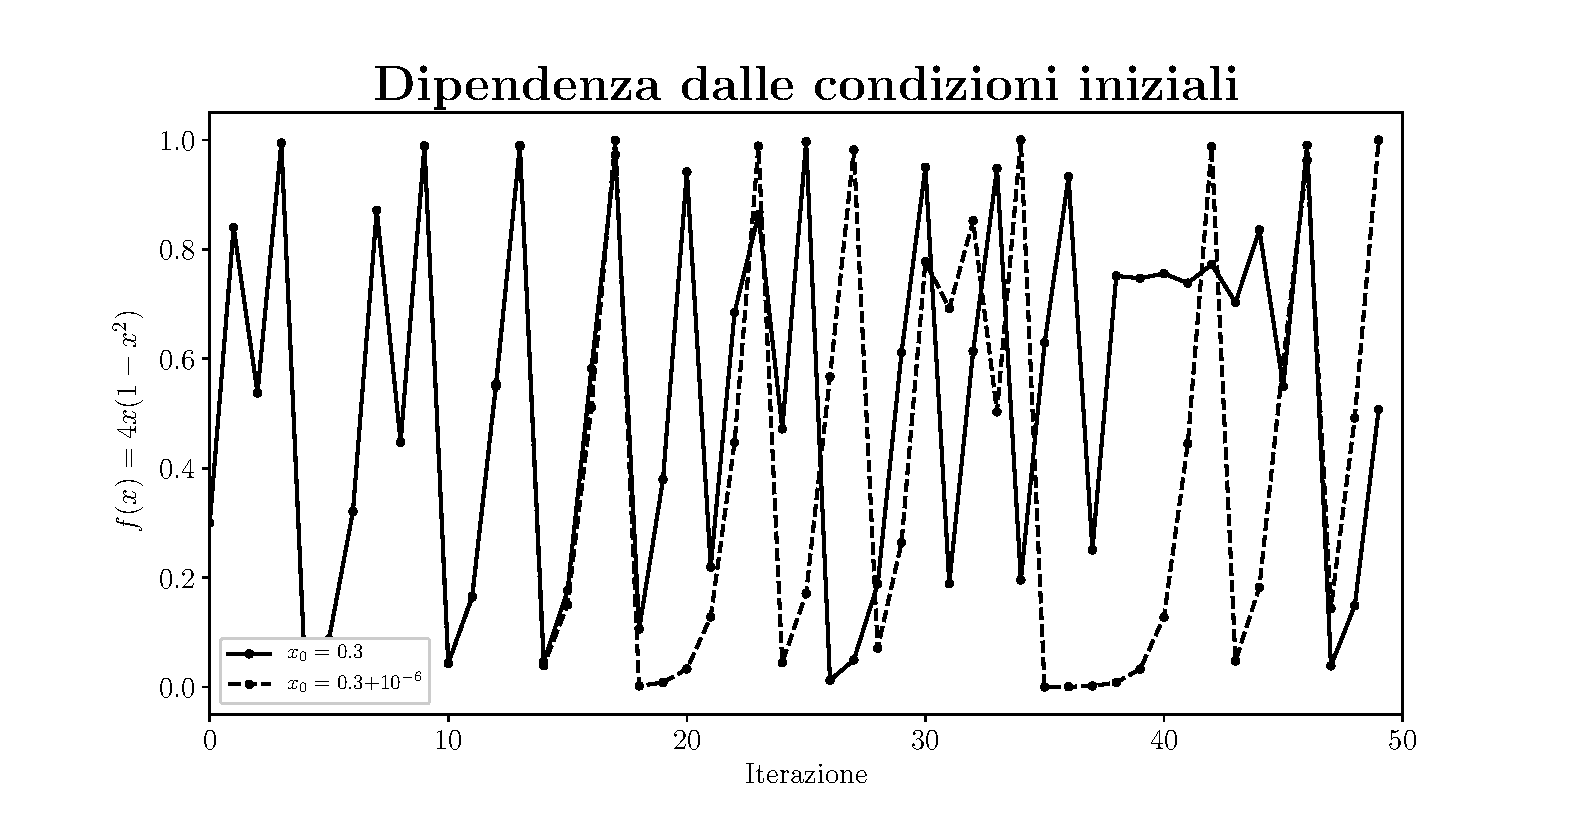
\includegraphics[scale=0.5]{Immagini/caos.eps}}
\end{minipage}   

\captionsetup{width=.8\linewidth}
\captionof{figure}{Sull'asse delle ascisse è riportato il numero dell'iterazione corrente della funzione logistica, sull'asse delle ordinate sono riportati gli stati alla $k$-esima iterazione di due evoluzioni partite una dal valore $x_0$, l'altra dal valore $x_0 + \epsilon$, dove si è scelto in questo caso $\epsilon = 10^{-6}$. Dopo alcune interazioni le due evoluzioni differiscono fortemente e non si trova più alcuna analogia tra esse.}
\label{fig:caos}
\vspace{20pt}

Questo fenomeno, vale a dire la forte dipendenza dai valori iniziali, è una delle caratteristiche principali dei fenomeni caotici, che di solito, quando insorgono, sono legati a dinamiche descritte da equazioni non lineari, come è infatti l'equazione logistica. Un esempio per visualizzare la forte dipendenza del sistema dalle considizioni iniziali è rappresentato nella figura \ref{fig:caos}, dove si sono scelti due valori iniziali distanti $\epsilon$ piccolo a piacere (nella figura $\epsilon = 10^{-6}$), e si sono tracciate le evoluzioni dell'equazione logistica a partire da essi. Si vede chiaramente che, dopo una decina di iterazioni, le due evoluzioni iniziano a differire sensibilmente, evolvendo in modo del tutto diverso. Tale comportamento è tanto più accentuato quanto più $r$ si avvicina al valore 4, ovvero evoluzioni che partono da valori molto vicini iniziano a divergere tanto prima, quanto più il valore di $r$ è grande.



\subsection{Non solo caos: isole di periodicità}
\begin{figure}[h!]
    \begin{center}  
    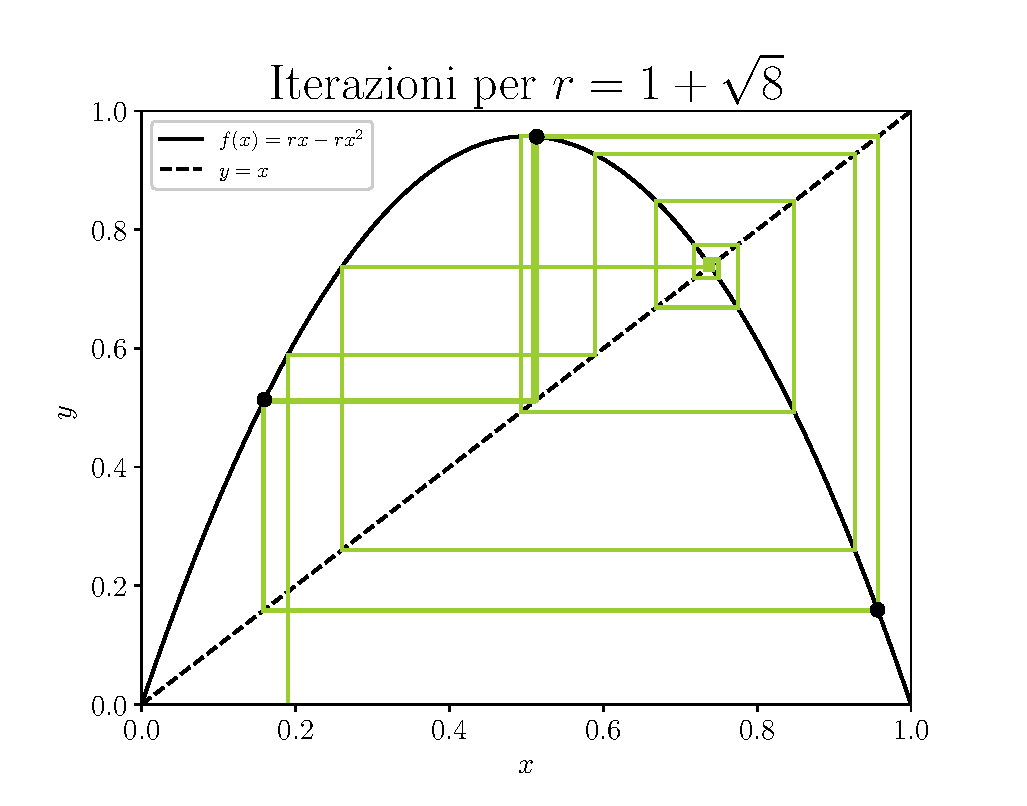
\includegraphics[scale=0.6]{Immagini/3_oscillazioni.eps} 
    \captionsetup{width=.8\linewidth}
    \caption{Oscillazione del sistema tra tre valori. Si può osservare che per $r = 1 + \sqrt{8}$, dopo un certo numero di iterazioni iniziali il sistema si assesta a oscillare tra 3 valori, che sono quelli sul grafico di $f$ per cui la linea verde risulta più spessa.}
    \label{fig:tre_osc}
    \end{center}   
\end{figure}
Si può pensare che, superato il valore $r_c$, il comportamento della mappa logistica continui semplicemente a essere caotico, ma in realtà si trova un altro fenomeno davvero interessante: per certi valori di $r$ si trova che la mappa logistica ritorna a oscillare periodicamente, ma stavolta non tra $2^k$ stati, bensì tra un numero dispari di stati. Ad esempio, per $r = 1 + \sqrt{8}$ il sistema oscilla periodicamente tra 3 valori, come mostrato dalla figura \ref{fig:tre_osc}.

In realtà un teorema, detto \textit{teorema di Sharowskii}, prevede che per ogni $N \in \mathbb{N}$ esista un valore di $r$ ammissibile per il quale il sistema oscilla tra $N$ valori. In pratica, quindi, nell'intervallo tra $r_c$ e 4 il caos è inframezzato da infinite "isole di periodicità", nelle quali il sistema torna ad assumere un carattere oscillatorio, ogni volta tra un numero diverso di stati. È assai celebre la rappresentazione grafica di questo comportamento nel cosiddetto "albero di Feigenbaum", nel quale vengono rappresentati sulle ascisse i valori che può assumere $r$, mentre sulle ordinate i valori asintotici del sistema dopo un numero infinito di iterazioni. Se il sistema ha un solo punto fisso attrattore, nel grafico sarà presente un solo punto, come si osserva infatti per $r<3$, mentre se il sistema oscilla tra più stati diversi, si fa "dividere" il grafico tra di essi. Il risultato è rappresentato nella figura \ref{fig:feigenbaum}.

\begin{minipage}{\linewidth}
\makebox[\linewidth]{
    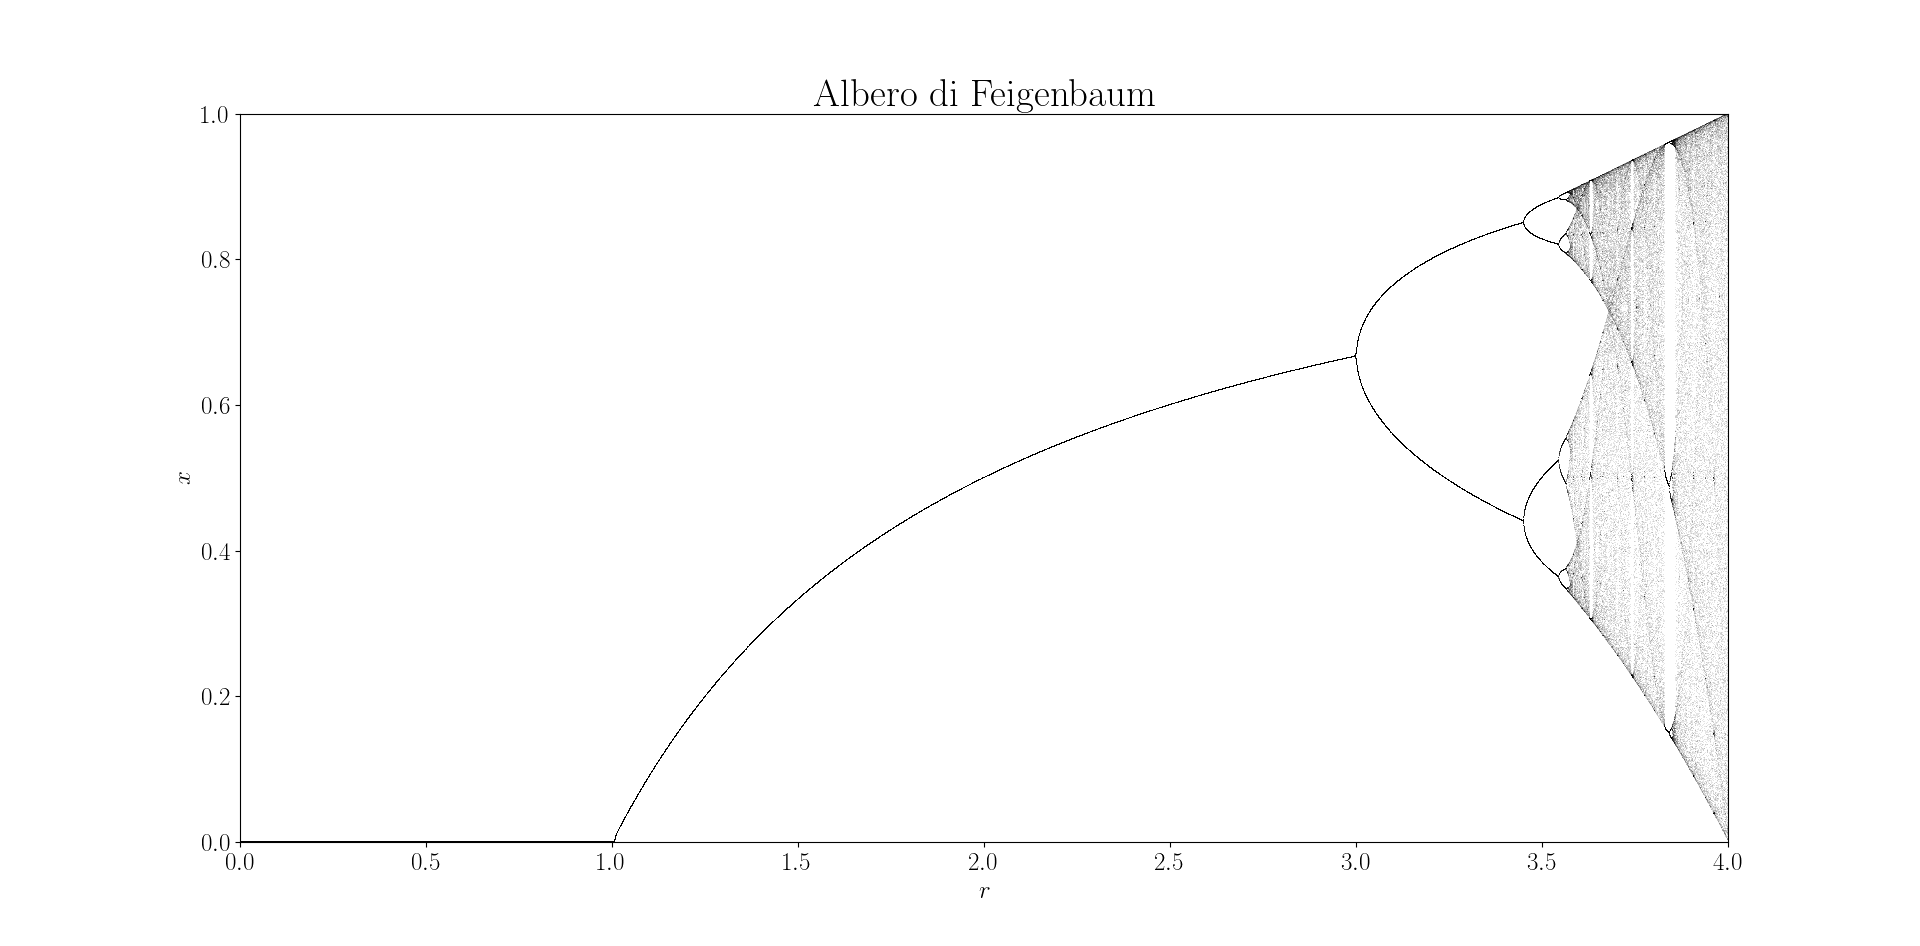
\includegraphics[scale=0.35]{Immagini/feigenbaum.png}}
\end{minipage}
\captionsetup{width=.8\linewidth}
    \captionof{figure}{L'albero di Feigenbaum rappresenta sulle ascisse i valori di $r$ e sulle ordinate i valori asintotici del sistema. Gli sdoppiamenti del grafico indicano che il sistema passa dal convergere a un valore all'oscillare tra più valori. Come si nota, dopo $r=3$ il sistema inizia a raddoppiare il proprio periodo di oscillazione fino al valore $r_c \simeq 3.56995$. Dopo di questo, però, si trovano ancora degli stati oscillatori, come quello molto ben visibile tra tre stati, per $r \simeq 1.8$.}
    \label{fig:feigenbaum}
